\documentclass[11pt,a4paper]{article}
\usepackage{polski}
\usepackage[utf8]{inputenc}
\usepackage{geometry}
\usepackage{graphicx}
\usepackage[dvipsnames]{xcolor}

\newgeometry{tmargin=3cm, bmargin=3cm, lmargin=1cm, rmargin=1cm}

\title{Testy aplikacji}
\author{Damian Rakowski 209300}
\date{29 maj 2019}




\begin{document}
\maketitle
\section{Wygląd aplikacji}
\begin{figure}[h]
\centering
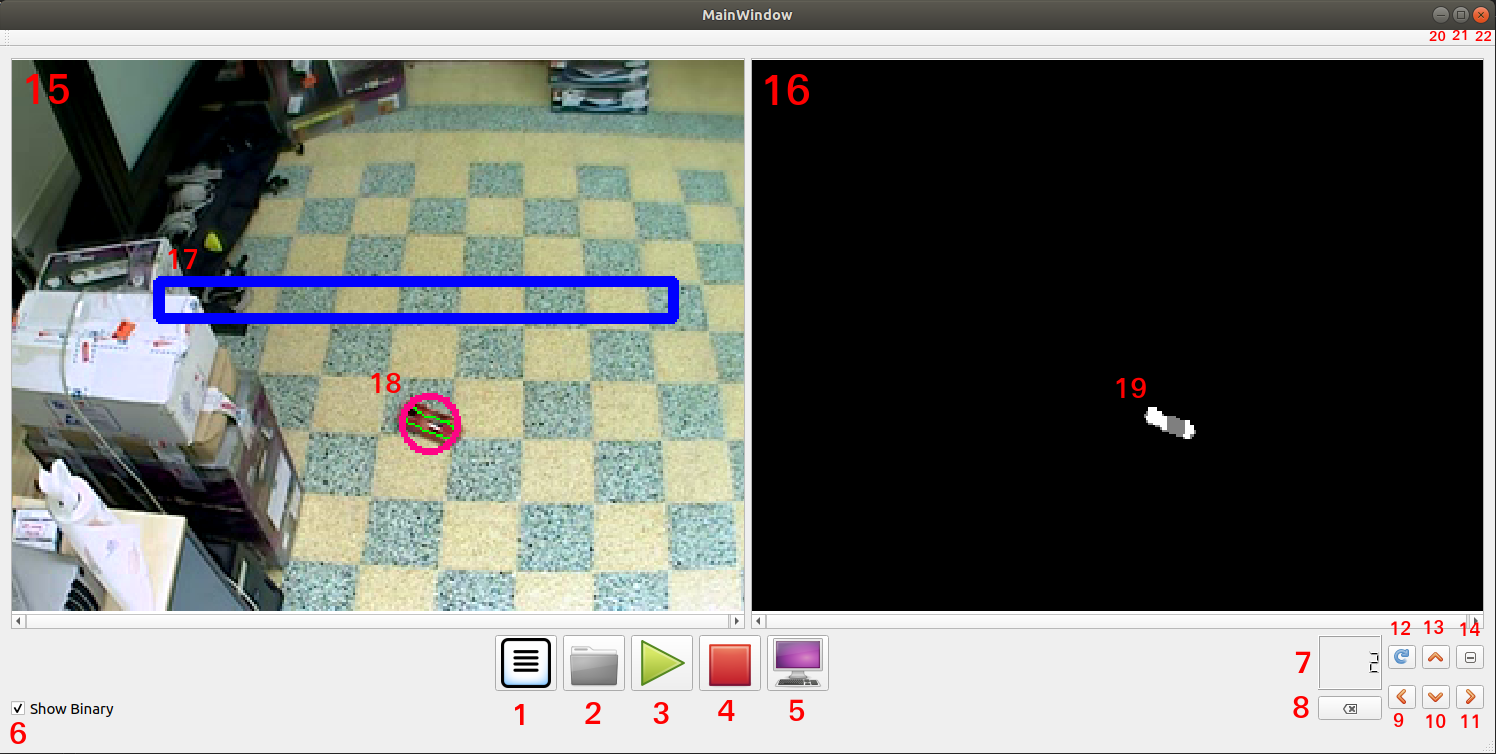
\includegraphics[width=\textwidth]{aplikacja.png}
\caption{Aplkiacja główna}
\vspace{1.5cm}
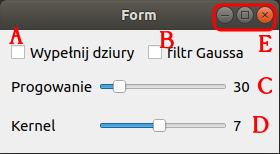
\includegraphics[scale=1]{opcje.png}
\caption{okienko z opcjami algorytmu}
\end{figure}

\section{Funkcjonalności do przetestowania manualnego}
\begin{enumerate}
\item[1] aplikacja wczytuje tylko pliki wideo i wyświetla ostrzeżenie jeżeli próbowano wczytać plik inny niż wideo
\item[2] wczytywanie/uruchamianie/wstrzymywanie/zamykanie pliku wideo (2,3,4)
\item[3] aplikacja wykrywa ruchome obiekty na obrazie
\item[4] wykryty  obiekt na obrazie jest opisany na  różowym kręgu oraz wyświetlane są jego krawędzie w kolorze zielonym (15,16)
\item[5] otwieranie/zamykanie obrazu binarnego (16)
\item[6] przetwarzanie pliku z kamery internetowej (5)
\item[7] otwieranie/zamykanie widżetu z parametrami algorytmu (1)
\item[8] zmiana położenia/rotacji/długości bramki wirtualnej przyciskami (12,13,14,9,10,11,17)
\item[9] zmiana położenia/rotacji/długości bramki wirtualnej klawiszami A/W/S/D/R/T
\item[10] bramka zlicza ruchomy obiekt, który przejechał przez bramkę i wyświetla wynik w 7.
\item[11] bramka zmienia kolor w zależności od wykrytego obiektu w środku
\item[12] aplikacja główna przed zamknięciem zamyka otwarty widżet z opcjami
\item[13] zamykanie/minimalizowanie/zmiana rozmiaru aplkiacji (20/21/22)
\item[14] przycisk 8 resetuje licznik bramki, który zaczyna od wartości 0
\item[15] algorytm wypełnia dziury (A)
\item[16] alorytm stosuje algorytm gaussa (B)
\item[17] algorytm ustawia wartośc progowania (C)
\item[18] alorytm umożliwia ustawienie rozmiaru jądra (D)
\item[19] okienko z opcjami algorytmu można zamknąć/rozwinąć/zminimalizować/ zmienić rozmiar
\item[20] przycisk numer 3 zmienia swoją ikonę. Zielony prostokąt jeżeli wczytano plik i jest zatrzymany. Szara ikona pauzy jeżeli wczytano plik i jest uruchomiony.
\end{enumerate}

\section{Funkcjonalności do przetestowania automatycznego}
\begin{itemize}
\item ustawianie parametrów aplikacji w dodatkowym widżecie
\end{itemize}

\section{Testy manualne}
\begin{enumerate}
\item[1] Aplikacja wczytuje pliki wideo i nie pozwala wczytać plików innego. Jeżeli spróbowano wczytać plik inny niż wideo, to wyskoczyło okienko z odpowiednią informacją o niepowodzeniu operacji.  \textcolor{red}{BŁĄD- Jeżeli zamkniemy krzyżykiem okno wyboru pliku, to wyswietli  sie informacja o nieudanej próbie wczytania pliku.}
\item[2] Aplikacja poprawnie wczytuje, uruchamia, wstrzymuje oraz zamyka plik wideo. Przyciski 2,3,4 działają poprawnie.
\item[3] Algorytm nie działa poprawnie w każdych warunkach. Szybkie zmiany oświetlenia, cienie  rzucane przez ruchome przedmioty oraz odbicia światła mogą zostać oznaczone jako ruchomy obiekt. 
\item[4] Każdy  wykryty obiekt jest opisany na różowym okręgu oraz jego krawedzie są zielone
\item[5]  Aplikacja poprawnie otwiera oraz zamyka obraz binarny
\item[6]  \textcolor{red}{Funkcjonalność nie działa}
\item[7] \textcolor{red}{ Przycisk numer 1 otwiera okno z parametrami ale go nie zamyka.}
\item[8] Przyciski 9 - 14 poprawnie sterują położeniem bramki na obrazie.
\item[9] Klawisze W/S/A/D/R/T poprwanie sterują położeniem bramki na obrazie
\item[10] Na podstawie analizy filmu testowego "car-over..." można stwierdzić że bramka wirtualna poprawnie zlicza wykryte obiekty, które z niej wyjadą. Wynik zostaje poprawnie wpisany do obiektu nr 7.
\item[11] Bramka poprawnie zmienia kolor. Bramka jest niebieska jeżeli jest pusta. Bramka jest zielona jeżeli w środku jest wykryty obiekt.
\item[12] \textcolor{red}{funkcjonalność nie działa}
\item[13] Przyciski 20,21,22 działją poprawnie. Można zmieniać rozmiar rozmiar aplikacji. \textcolor{yellow}{Przy pewnym rozmiarze okienko 15 i 16 zaczyna samoczynnie synchronicznie zmieniać swój rozmiar.}
\item[14] Przycisk numer 8 poprawnie resetuje licznik
\item[20] Przycisk numer 3 poprawnie zmienia swoją ikonę w zależności od stanu odtwarzania i wczytania pliku wideo.


\end{enumerate}



\end{document}
